%% FSE (CS-5187 Term Project) research paper. Requirements from the CFP (https://conf.researchr.org/home/fse-2026, checked 2026-09-30):
%%   * \documentclass[acmsmall,screen,review,anonymous]{acmart}; single column
%%   * 12 pages of text and figures + references limit \todo{check}
%%   * double-anonymous: no names, no identifying URLs, third-person
%%     self-citation, no acknowledgments at submission
%%   * "Data Availability" section after the Conclusion (not counted)
%%   * disclose AI tools; fabricated citations = desk reject
%%   * deadline: TODO (see course page) AoE, TODO
%% Used for e.g. FSE, ISSTA, OOPSLA/PACMPL, TOSEM.
\documentclass[acmsmall,screen,review,anonymous]{acmart}

%% Shared macros. Keep notation here so the paper cannot drift from itself.
%% Rule: every name, symbol and set used more than once gets a macro here.
\usepackage{amsmath}
\usepackage{booktabs}
\usepackage{xspace}
\usepackage{listings}
\usepackage{xcolor}
\usepackage{array}
\usepackage{pifont}
\usepackage{tikz}
\usetikzlibrary{arrows.meta,positioning,calc,fit,backgrounds}
\DeclareRobustCommand{\circled}[1]{\tikz[baseline=(c.base)]\node[circle,draw,inner sep=0.7pt,font=\tiny\bfseries] (c) {#1};}

% ---- project name (anonymised for review) ----
% Works for any CS-5187 project: a tool, a technique/method, or an empirical
% study. With no tool (e.g. a study), read \tool as "our study" and reword
% "We present \tool" -> "We study ...", "\tool records" -> "our method ...".
\newcommand{\tool}{\textsc{YourTool}\xspace}   % TODO: final name (tool, method, or study)

% ---- notation (one macro per symbol; comment says what it means) ----
% \newcommand{\Seen}[1]{\ensuremath{\mathit{Seen}(#1)}} % example: lines the compiler sees

% ---- research questions ----
\newcommand{\rqref}[1]{\textbf{RQ#1}\xspace}

% ---- results: one boxed, numbered claim per observation ----
\newcounter{observation}
\newsavebox{\obsbox}
\newenvironment{observation}
  {\refstepcounter{observation}\par\smallskip\noindent\begin{lrbox}{\obsbox}\begin{minipage}{0.95\linewidth}\textbf{Observation~\theobservation.}~}
  {\end{minipage}\end{lrbox}\fbox{\usebox{\obsbox}}\par\smallskip}

% ---- CS-5187 term-project FOCUS callouts (RED, on purpose) ----
% A red box that marks a part every term-project report MUST address:
%   Research Questions, Motivating Example, Workflow, Related Work,
%   Threats to Validity. The red is a study aid, not paper style -- once
%   you have written the section, DELETE its \focus{...} line (keep the
%   section). A finished report has zero \focus and zero \todo.
\newcommand{\focus}[1]{%
  \par\smallskip\noindent
  {\color{red}\rule{\linewidth}{0.6pt}}\par\nobreak\vspace{1pt}\noindent
  {\color{red}\ding{228}~\textbf{FOCUS --- graded, must address:}~\itshape #1}\par\nobreak\vspace{1pt}
  {\color{red}\rule{\linewidth}{0.6pt}}\par\smallskip}

% ---- editorial (all must be gone before submission; scripts/check.sh counts them) ----
\newcommand{\todo}[1]{\textcolor{red}{[TODO: #1]}}
\newcommand{\num}[1]{\textcolor{blue}{#1}}   % a number not yet measured by the final tool
\newcommand{\cmark}{\ding{51}}
\newcommand{\xmark}{\ding{55}}

\lstset{basicstyle=\ttfamily\footnotesize,columns=fullflexible,
        keepspaces=true,frame=single,framesep=2pt,xleftmargin=4pt,
        numbers=left,numberstyle=\tiny,numbersep=4pt}

% long \texttt words otherwise run into the margin
\setlength{\emergencystretch}{3em}


\setcopyright{none}
\acmConference[FSE (CS-5187 Term Project)]{ACM International Conference on the Foundations of Software Engineering (Format Template)}{2026}{IIT Guwahati}
\acmYear{2026}
\citestyle{acmauthoryear}

\begin{document}

\title[Check the Tree]{Check the Tree: Finding Wrong Results in PostgreSQL with Typed Derivation Trees and Commit-Directed Grammar Extension}
%% Alternative titles (keep 2-3 here until submission):
%%   "Rewrite the Tree, Not the Text: Grammar-Aware Metamorphic Fuzzing of PostgreSQL"
%%   "Grow the Grammar from the Commit: LLM-Guided, Oracle-Rich Fuzzing of PostgreSQL"

\author{Anonymous Author(s)}
\affiliation{\institution{Anonymous Institution}\country{Anonymous Country}}

\begin{abstract}
%% LENGTH: with the result tables the main text must still be cut to 12 pages
%% (FSE limit): candidates are the component table and the oracle list.
%% ABSTRACT (150-250 words, one paragraph, no citations, no \ref).
%% Pattern (from earlier papers):
%%  1. The problem in 2-3 short sentences. Plain words; what tools do today.
%%  2. Why it matters: ONE concrete, real case with an exact number
%%     (e.g. a CVE, a miscompilation, a measured share).
%%  3. "We present \tool." What it does, in steps, in one or two sentences.
%%  4. Results with numbers: "On X, \tool ... from A\% to B\%."
%%  5. One honest lesson or surprise the work taught ("The run also shows ...").
%% No "novel", no "we propose a framework", no promises without numbers.
\todo{Problem in two sentences.} \todo{One real case with a number.}
We present \tool. \todo{What it does.} \todo{Results with numbers.}

\end{abstract}

%% CCS concepts: pick the ones that fit YOUR project at https://dl.acm.org/ccs
%% (500 = main, 300 = secondary). This template fits any software-engineering
%% topic -- static analysis, dynamic analysis/testing, empirical studies,
%% program repair, tools, human factors, etc. -- so replace the placeholder
%% below with the concept for your own work. A few common top-level ids:
%%   Software and its engineering~Software testing and debugging
%%   Software and its engineering~Automated static analysis
%%   Software and its engineering~Dynamic analysis
%%   Software and its engineering~Software creation and management
%%   General and reference~Empirical studies
\begin{CCSXML}
<ccs2012>
  <concept>
    <concept_id>10011007.10011074.10011099.10011102.10011103</concept_id>
    <concept_desc>Software and its engineering~Software testing and debugging</concept_desc>
    <concept_significance>500</concept_significance>
  </concept>
  <concept>
    <concept_id>10002951.10002952</concept_id>
    <concept_desc>Information systems~Data management systems</concept_desc>
    <concept_significance>300</concept_significance>
  </concept>
</ccs2012>
\end{CCSXML}
\ccsdesc[500]{Software and its engineering~Software testing and debugging}
\ccsdesc[300]{Information systems~Data management systems}

\keywords{fuzzing, database testing, test oracles, metamorphic testing,
  grammar-based testing, large language models, PostgreSQL}

\maketitle

\section{Introduction}
\label{sec:intro}

Suppose you run a reporting query on \pg and it returns a row that should not
be there. The query does not crash and no error is raised. Nothing in the
logs says that the answer is wrong. This kind of failure, a \emph{wrong
result}, is the most harmful bug a database system can have, because the user
has no way to notice it.

Fuzzers for database systems mostly look for crashes. SQLsmith~\cite{sqlsmith}
generates random queries from the system catalog, and
SQUIRREL~\cite{zhong2020squirrel} mutates SQL with coverage feedback. Both
detect a bug when the server crashes or an assertion fails. To find wrong
results, a fuzzer needs a \emph{test oracle} that knows the right answer.
Differential testing compares two systems~\cite{slutz1998rags}; metamorphic
oracles such as Ternary Logic Partitioning (TLP)~\cite{rigger2020tlp},
NoREC~\cite{rigger2020norec} and equivalent expression
transformation~\cite{jiang2024eet} compare a query with a rewritten query that
must return the same rows. These oracles rewrite the SQL text of a query,
so each tool builds its own small query generator that the oracle understands.

We focus on a gap between the two lines of work. Grammar-based generators
reach deep into the planner but do not know which parts of a query can be
rewritten safely. Oracle-based tools know how to rewrite, but their
generators cover a small part of SQL. And neither knows what changed in the
code yesterday: the planner of \pg master changes every week, and most new
bugs live in the newest code.

Figure~\ref{fig:motivating} shows a real wrong result that \tool found. Since
\pg~17, the planner replaces \texttt{range @> elem} by the constant
\texttt{true} when the range is unbounded on both sides, and by
\texttt{false} when it is empty. The operator is strict, so for a NULL
element the correct answer is NULL. The constant is wrong under \texttt{NOT},
in \texttt{IS NULL} tests, in \texttt{CASE}, and in outer joins, where unmatched
rows carry NULLs. We reproduced the bug on the release 18.6 and on master.
\tool found it with a typed rewrite of the derivation tree (a scalar
subquery around the range), in the first 150 test cases the rewrite ran.

This is not a single case. Between 31~July and 16~October~2026, \pg master
received 23 fixes in query processing that came with a regression test and
still revert cleanly (Section~\ref{sec:rq3}). When we put each bug back, 20 of
them change what a query returns: 8 return wrong rows, 5 raise internal
errors, 4 fail an assertion, and 3 raise or drop an error message. Only 9 of
these 20 can be seen by a crash-only fuzzer.

\begin{figure}[t]
\begin{lstlisting}[numbers=none,escapechar=!,language=SQL]
SELECT c,
       '(,)'::int4range @> c       AS contains,   -- must be NULL when c is NULL
       NOT ('empty'::int4range @> c) AS not_empty  -- must be NULL when c is NULL
FROM (VALUES (NULL::int), (1)) v(c);

  c   | contains | not_empty
------+----------+----------
 NULL | t        | t          !\textbf{$\leftarrow$ wrong: the planner folded the call to a constant}!
 1    | t        | t
\end{lstlisting}
\caption{A wrong result in \pg~17, 18.6 and master that \tool found: the
planner support function for range containment returns \texttt{true} or
\texttt{false} for a NULL element, where the strict operator gives NULL. No
error or crash shows it; only an oracle that compares two equivalent queries
does.}
\label{fig:motivating}
\end{figure}

Closest to us is query plan guidance~\cite{ba2023qpg}, which steers a
generator toward new plan shapes, and Fuzz4All~\cite{xia2024fuzz4all}, which
uses a large language model (LLM) as the generator. However, plan guidance
uses the oracles of SQLancer and their small query language, and an LLM that
writes every test case is slow and produces many invalid queries. Neither
connects the generator to the code that changed.

We present \tool, a grammar-aware fuzzer for \pg built on three ideas:
\begin{enumerate}
  \item A \emph{typed grammar} generates SQL as derivation trees. Every node
    knows its type and its place in the query (Section~\ref{sec:grammar}).
  \item \emph{Tree-based oracles} rewrite the derivation tree, not the text:
    TLP on \texttt{WHERE} and \texttt{HAVING} at any query level, NoREC, ten
    typed expression rewrites, CTE materialisation and table fences. A
    plan-variant oracle and a cross-version oracle compare the same query
    under other planner settings and on the last release
    (Section~\ref{sec:oracles}).
  \item \emph{Commit-directed grammar extension}: an LLM reads a recent commit
    and proposes grammar alternatives and seed queries; a \gate accepts them
    only if the server runs them and they execute the lines the commit
    changed (Section~\ref{sec:llm}).
\end{enumerate}
\tool then reduces every finding to a short reproducer and records a verdict
for it (Section~\ref{sec:triage}).

\num{First results.} In a four-minute smoke run on a server with the 23 bugs
put back, \tool rediscovered an assertion failure in \texttt{JSON\_TABLE}
that we had found earlier on master, and its triage exposed two false-positive
classes in our own oracles, which we fixed (Section~\ref{sec:rq2}).
\num{RQ1--RQ4 numbers follow from the full campaigns.} The lesson so far is
that oracle precision, not generator power, limits a wrong-result fuzzer: a
generator that reaches more of SQL also reaches more corner cases where two
``equivalent'' queries are not equivalent.

\paragraph{Contributions.}
\begin{itemize}
  \item A typed SQL grammar for \pg with node spans, so that oracles can
    rewrite derivation trees (Section~\ref{sec:approach}).
  \item Six metamorphic oracles on derivation trees, plus plan-variant and
    cross-version oracles, with the precision of each (Section~\ref{sec:rq2}).
  \item A commit-directed LLM extension with a \gate that checks validity,
    reachability and diff coverage on the server (Section~\ref{sec:llm}).
  \item A benchmark of 23 real \pg bugs put back into one server, with a
    single-bug server per bug for attribution (Section~\ref{sec:rq3}).
  \item Two previously unknown \pg bugs, one wrong result and one assertion
    failure, with patches (\num{upstream status}; Section~\ref{sec:rq2}), and
    the tool and all data (Section~\ref{sec:data}).
\end{itemize}

\section{Background}
\label{sec:background}

\paragraph{Derivation tree.} A grammar derives a query by choosing one
alternative per rule. The \emph{derivation tree} \Tree{\Q} of a query \Q
records these choices: each inner node is a rule with the alternative it took,
and the leaves are SQL tokens. Reading the leaves from left to right gives the
text of \Q.

\paragraph{Wrong result.} A query has a wrong result when the server returns a
multiset of rows \Res{\Q} that differs from what the SQL standard and the \pg
documentation define, without an error. Typical causes are planner rules that
are correct only under an assumption that does not hold, for example that a
column cannot be NULL.

\paragraph{Metamorphic oracle.} A metamorphic oracle builds a second query
$\Q'$ with a known relation to \Q, usually $\Res{\Q} = \Res{\Q'}$, and reports a
bug when the relation fails. TLP~\cite{rigger2020tlp} uses
$\Res{\Q} = \Res{\Part{\Q}{p}} \uplus \Res{\Part{\Q}{\neg p}} \uplus
\Res{\Part{\Q}{p \;\mathtt{IS\;NULL}}}$ for a predicate $p$ added to
\texttt{WHERE}. NoREC~\cite{rigger2020norec} compares the row count of
\texttt{SELECT * FROM t WHERE p} with the number of rows on which $p$ is true
when $p$ is evaluated in the select list, where the planner cannot use it to
choose a plan.

\paragraph{Plan variant.} \pg lets a session switch planner methods off, for
example \texttt{SET enable\_hashjoin = off}. A \emph{plan variant} is the
same query under such a setting. All plan variants of a deterministic query
must return the same multiset. This is differential testing inside one
server.

\paragraph{Assertion build.} \pg built with \texttt{--enable-cassert} checks
internal invariants with \texttt{Assert}. A failed assertion aborts the backend
and prints a \texttt{TRAP} line with the file and the expression to the
server log. Release builds skip these checks, so an assertion failure often
corresponds to silent corruption or a wrong result in production.

\section{Problem Statement}
\label{sec:problem}

Let $G$ be a typed grammar for the SQL dialect of \pg and $S$ a database
schema. A \emph{test case} is a sequence of statements derived from $G$ over
$S$, run in one transaction that is rolled back at the end. The
\emph{derivation tree} \Tree{\Q} of a query \Q records the alternative each rule
took; its leaves, read left to right, are the text of \Q. A query has a
\emph{wrong result} when the server returns, without an error, a multiset
\Res{\Q} that differs from what the SQL standard and the \pg documentation
define. An \emph{oracle} maps the server's response to a test case to
\emph{pass} or \emph{bug candidate}: a metamorphic oracle such as
TLP~\cite{rigger2020tlp} or NoREC~\cite{rigger2020norec} compares \Q with a
rewritten query, and a \emph{plan variant} (the same query under a setting such
as \texttt{SET enable\_hashjoin = off}) must return the same multiset.

\paragraph{Sound rewrites.} A tree rewrite $r$ maps \Tree{\Q} to a second
tree. It is \emph{sound} for \Q if $\Res{\Q} = \Res{r(\Q)}$ holds on every
correct server. A rewrite that is sound only under conditions (for example,
only if no \texttt{LIMIT} without \texttt{ORDER BY} appears below the rewritten
node) must check them on the tree before it is applied. An unsound rewrite
produces \emph{false positives}: candidates that are not bugs.

\paragraph{Goal.} Given a fixed time budget $B$ and one server, find as many
distinct bugs as possible, where a bug is a crash, a failed assertion, an
internal error (SQLSTATE class \texttt{XX}), or a wrong result, while keeping
the \emph{precision} of each oracle high:
\begin{equation}
  \mathit{precision}(o) = \frac{|R_o|}{|R_o| + |F_o|}
  \label{eq:precision}
\end{equation}
where $R_o$ and $F_o$ are the real bugs and the false positives among the
distinct candidates oracle $o$ reported, after de-duplication by signature
(Section~\ref{sec:triage}). Candidates that do not reproduce (flaky) are
counted apart, and a duplicate of a bug reported upstream is a real bug that
we report separately, so we also give precision with duplicates in $R_o$.

\paragraph{Why not let an LLM write the test cases?} An LLM can write SQL that
targets a feature, but at a few seconds per call it writes at most a few
thousand test cases in an hour, where the grammar arm produced 71{,}228
(Table~\ref{tab:rq1}). LLM-written queries are also not derivation trees, so
the tree-based oracles cannot rewrite them. We use the LLM to extend the grammar
instead: a few calls per commit, after which the grammar generates thousands of
variations.

\section{Approach}
\label{sec:approach}

Figure~\ref{fig:overview} shows the steps of \tool. The main idea is to keep
every generated query as a typed derivation tree until it has been run, so
that oracles can rewrite single nodes of known type and position instead of
SQL text. The tree has four jobs: generation builds it, mutation re-derives
one subtree, the oracles rewrite one typed node, and triage reduces it by
replacing subtrees with their smallest derivation. The fuzzing loop (Steps
1--4) runs thousands of test cases per minute; the LLM loop (Step 5) runs a few
times per commit, before the campaign.

\begin{figure*}[t]
  \centering
  %% Figure: overview of the tool. Steps left to right, loop dashed.
%% Grayscale-safe (black lines, black!6 fill), \scriptsize text, numbered
%% steps matching the "Step N" subsections.
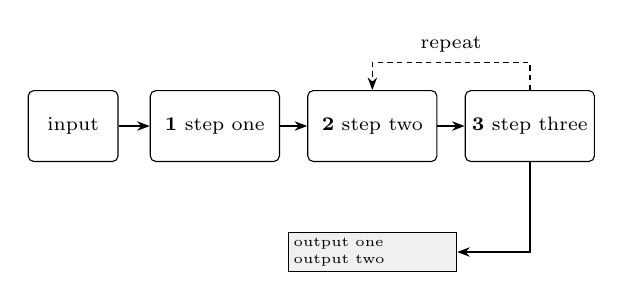
\begin{tikzpicture}[
    x=1cm, y=1cm, font=\scriptsize,
    box/.style={draw, rounded corners=2pt, align=center, inner sep=2pt,
                minimum height=9mm, text width=15mm, fill=white},
    outbox/.style={draw, align=left, inner sep=2pt, fill=black!6,
                text width=20mm, font=\tiny},
    flow/.style={-{Stealth[length=1.6mm]}, line width=0.5pt},
    back/.style={-{Stealth[length=1.6mm]}, line width=0.5pt, dash pattern=on 2pt off 1.5pt},
  ]
  \node[box, text width=10mm] (in) at (0,0) {input};
  \node[box] (s1) at (1.8,0) {\textbf{1} step one};
  \node[box] (s2) at (3.8,0) {\textbf{2} step two};
  \node[box] (s3) at (5.8,0) {\textbf{3} step three};
  \node[outbox] (o) at (3.8,-1.6) {output one\\output two};
  \draw[flow] (in) -- (s1);
  \draw[flow] (s1) -- (s2);
  \draw[flow] (s2) -- (s3);
  \draw[flow] (s3.south) |- (o.east);
  \draw[back] (s3.north) -- ++(0,0.35) -| node[pos=0.25, above] {repeat} (s2.north);
\end{tikzpicture}

  \caption{Overview of \tool. The top row is the fuzzing loop: test cases are
  derived from the typed grammar, oracles are attached as rewrites of the
  derivation tree, and the server runs each query under several settings.
  The bottom row runs before a campaign: an LLM turns a recent commit into
  grammar alternatives, and the \gate accepts them only when the server runs
  them and they reach the changed lines.}
  \label{fig:overview}
\end{figure*}

\subsection{Step 1: Derive Test Cases from a Typed Grammar}
\label{sec:grammar}

We wrote a grammar for the SQL that \pg~18 and master accept, in a small format
of our own (\pgg): 78 rules with 421 alternatives over 13 SQL types. A rule may
be parameterised by a type, as in \texttt{expr<T>}, so a derivation only
combines expressions that type-check. Weights set how often each alternative is
chosen, and \emph{builtins} written in Python handle what a context-free
grammar cannot: \texttt{@col(T)} picks a visible column of type $T$ in the
current scope, \texttt{@table} binds a fresh alias, and \texttt{@group\_keys}
makes the current query level grouped, after which only grouped columns and
aggregates are visible. The schema has 9 relations with partitions, inheritance,
a view, indexes of four access methods and NULLs in most columns.

A test case has up to two setup statements (DDL, DML, \texttt{ANALYZE},
\texttt{SET LOCAL} of a planner setting) followed by one or two queries. While
deriving, the engine wraps the tokens of every node in invisible markers, so
after rendering it knows the exact token span of each node. Half of the test
cases are new derivations; the others replay a corpus test case and re-derive one
subtree. A test case enters the corpus when it produces a new bug signature, a
new SQL feature, a new pair of features, or a new plan shape, the digest of the
node types in \texttt{EXPLAIN} output~\cite{ba2023qpg}.

\paragraph{Feedback and data.} Every alternative carries a multiplicative
weight that grows when a test case that used it enters the corpus and shrinks
when its statement fails (rate $\eta=0.1$, range $[0.2,5]$). Some literals come
from a \emph{data profile} (minimum, maximum and quantiles of every column,
type edges such as $-0$, NaN, $\pm$Infinity and the empty array), so predicates
select a real share of rows. Grammar-based generation is not new; the typing,
scoping builtins and node spans are what the later steps need.

\subsection{Step 2: Attach Oracles as Tree Rewrites}
\label{sec:oracles}

For each query, \tool picks up to one metamorphic check and stores it with
the test case as a pair of queries that must return the same multiset. All
checks are built on the derivation tree.

\paragraph{Partitioning and counting.} \emph{TLP on \texttt{WHERE}} picks a
\texttt{SELECT} whose result is used as a multiset (the query itself, a
derived table, a CTE body, a set-operation arm, or an \texttt{IN},
\texttt{EXISTS} or \texttt{LATERAL} subquery) and partitions its
\texttt{WHERE p} into $p$, \texttt{NOT p} and \texttt{p IS NULL}, combined
with \texttt{UNION ALL}. Because the rewrite edits one node, it also works in
a nested query, where text-based TLP does not apply. \emph{TLP on
\texttt{HAVING}} does the same; the unpartitioned side keeps \texttt{HAVING
TRUE}, because without \texttt{GROUP BY} a \texttt{HAVING} clause is what makes a
level a single-group aggregate. \emph{TLP on aggregates} equates a global
\texttt{MIN}, \texttt{MAX}, \texttt{SUM}, \texttt{COUNT}, \texttt{BIT\_*} or
\texttt{BOOL\_*} with the combination over the three partitions (the
\texttt{MIN} of the \texttt{MIN}s, the \texttt{SUM} of the \texttt{COUNT}s).
\emph{NoREC} compares \texttt{count(*)} with \texttt{WHERE p} against the sum
of \texttt{CASE WHEN p THEN 1 ELSE 0 END}.

\paragraph{Equivalent forms of one node.} \emph{Expression rewrites} replace
one typed expression $e$ by \texttt{COALESCE(e,e)}, \texttt{(SELECT e)},
\texttt{CASE WHEN TRUE THEN e END}, $e+0$ or $e \cdot 1$ (numbers),
\texttt{e || ''} (text), or \texttt{NOT NOT p}, \texttt{p AND TRUE},
\texttt{p OR FALSE} (predicates). \emph{Predicate rewrites} turn
\texttt{x IN (a, b)} into \texttt{(x = a) OR (x = b)}, which \pg~18 turns back
into \texttt{= ANY}, \texttt{a < b} into \texttt{NOT (a >= b)}, which
three-valued logic keeps exact, and \texttt{BETWEEN} into two comparisons.
\emph{NOT NULL conjunct} turns \texttt{WHERE p} into \texttt{WHERE p AND c IS
NOT NULL} for a NOT NULL column $c$ that $p$ uses, which targets the planner's
NOT NULL simplifications; it is skipped under outer joins and for generated
columns, where such a column can still be NULL. \emph{ORDER BY removal} drops
the statement's own \texttt{ORDER BY}, \emph{CTE materialisation} toggles
\texttt{MATERIALIZED}, and the \emph{table fence} turns one table reference
into \texttt{(SELECT * FROM t OFFSET 0)}, which stops the planner from pushing
predicates into it, removing it, or pruning its partitions.

\paragraph{Security and estimates.} For \emph{row-level security}, five tables
carry a policy defined in one file used by both the server and the rewrite.
The query runs as a restricted role, under the policies, and as a superuser
with every protected table $t$ replaced by \texttt{(SELECT * FROM t WHERE
\textit{policy})}; a difference means that the policies let a row through or
hide one they should not. Following CERT~\cite{ba2024cert}, adding the
\texttt{WHERE} clause to a query must not raise the planner's row estimate;
this check compares \texttt{EXPLAIN} estimates, and a violation is a
\emph{performance} candidate, reported apart from bugs.

A check is attached only if its rewrite is sound for that query
(Section~\ref{sec:problem}).

\subsection{Step 3: Run the Test Case Several Ways}
\label{sec:run}

The server runs each test case in a transaction with one savepoint per
statement and rolls it back at the end, so test cases cannot affect each other.
For each deterministic query \tool also runs (i)~both sides of the attached
check; (ii)~the query under two of 18 \emph{plan variants} (for example hash
join only, no hash aggregation, forced parallel plans, partitionwise join, no
eager aggregation, JIT), chosen at random per query; and (iii)~the whole test
case on a server of the last release, \pg~18.6, in a database of its own for
each worker (the \emph{cross-version oracle}). Results are compared as
order-insensitive digests that drop choices no plan controls: trailing zeros of
equal \texttt{numeric} values, the sign of float zero, the last digits of finite
floats in aggregates, and the text of equal \texttt{interval} values.

\subsection{Step 4: Classify, De-duplicate, Triage}
\label{sec:triage}

The oracle reads the statement results and the server log. A \texttt{TRAP} line
is an assertion failure; a lost connection without one is a crash; an error of
class \texttt{XX} is an internal error; a confirmed mismatch of any digest is a
wrong result (a metamorphic mismatch counts only if it repeats when both sides
run again). Crash evidence counts only if it carries the process id of the test
case's own backend or its parallel workers. Each candidate gets a
\emph{signature}: the assertion location, the normalised backtrace or error
message, or, for wrong results, the oracle and the shape of the query; only the
first test case per signature is saved.

Triage reproduces the candidate three times on a fresh connection and reduces
it in two stages. \emph{Tree reduction} works on the derivation trees that every
failure of the grammar arm stores: it drops a statement, drops one repetition,
or replaces a subtree by the smallest derivation of the same rule and type, and
replays the trees through the generator, which re-binds names, aliases and
types. Every candidate is therefore valid SQL, and the server's time goes to the
question whether the failure remains. \emph{Token reduction} follows: delta
debugging~\cite{zeller2002dd} removes statements, then clauses, list items and
parenthesised groups level by level over the parenthesis
tree~\cite{misherghi2006hdd}, then single tokens. A step is kept only if the same
failure occurs (same assertion, normalised message, or oracle and plan variant);
for a metamorphic candidate both queries are reduced together, so they stay a
valid pair.

\paragraph{Localization.} For a reduced wrong result, \tool runs the queries
under every plan variant. If a variant removes the disagreement, the bug is in
the code path that setting switches, and the report names the setting and its
source files; if none does, the cause is an always-applied rewrite, constant
folding, a planner support function, or expression evaluation. The output is a
short reproducer, the rows each side returned, the localization and a draft
report in the shape of the \pg bug form.

\subsection{Step 5: Extend the Grammar from Recent Commits}
\label{sec:llm}

\paragraph{Step 5a: propose.} \tool lists the commits of \pg master that change
the optimiser, executor, parser or SQL-callable functions and add regression
tests. For each it builds a digest: the message, the changed functions, the SQL
the commit added to the tests, and the \emph{diff-coverage targets}, the changed
lines of each C file. An LLM gets the digest with a fixed, cached system prompt
(the \pgg format, the builtins, the conventions of the grammar, the schema and
the whole current grammar) and answers with structured output: a rationale, a
fragment of new alternatives, one to five seed test cases, the features it
targets, and up to three \emph{equivalence rewrites}, templates over one
expression of a given type such as \texttt{CASE WHEN \{e\} IS NULL THEN NULL
ELSE \{e\} END} that the model claims equal \texttt{\{e\}} for every value. The
commit miner never shows the model a fix that the benchmark of
Section~\ref{sec:rq3} reverts.

\paragraph{Step 5b: validate.} No model output reaches the campaign unless the
server agrees. The \gate checks in order: (i)~\emph{parse}: the fragment parses
with the grammar, adds no types and uses only known builtins;
(ii)~\emph{reachability}: in a sample of 150 test cases with the new alternatives
boosted, they are used at least five times; (iii)~\emph{validity}: at least 60\%
of the statements that use them run without error; (iv)~\emph{seeds}: each seed
runs; and (v)~\emph{diff coverage}: on a gcov build, the sample executes more of
the commit's changed lines than the same sample without the fragment. A failed
check sends its findings (the parse error, the most frequent error messages, the
uncovered lines) back to the model for up to three repair rounds; every round is
a ledger line with its tokens, cost and the gate's report.

A proposed rewrite is a claim about semantics, so the gate tests it twice. The
server evaluates \texttt{rewrite(v) IS NOT DISTINCT FROM v} for NULL, the edge
values of the type and quantiles of the data; then \tool applies the rewrite
alone to the expressions of 150 test cases, with confirmation re-runs. The
rewrite is accepted only if no value and no query shows a difference, and it
then becomes an expression rewrite of Step~2. Neither test varies the
collation, so the gate also rejects a template with an explicit
\texttt{COLLATE} (Section~\ref{sec:rq4}).

\section{Implementation}
\label{sec:impl}

\tool is about 10{,}500 lines of Python with 138 unit tests, plus the 628-line
grammar. It drives \pg through \texttt{psycopg}, reads the server log for
assertion and crash evidence, and runs every trial as a resumable process
whose events, timeline and failures are written as JSON. The parts are:
Its parts are the \pgg parser and derivation engine (scopes, type variables,
node spans, the \texttt{MINIMAL} marker); the generator (corpus, alternative
weights, data profile); the executor (savepoints, plan variants, metamorphic,
RLS and CERT checks, and a cross-version wrapper); triage (reproduction, tree
and token reduction, localization, reports, bisection, the precision ledger);
the benchmark scripts with \texttt{bench verify} and \texttt{bench attribute};
and the LLM arm (commit miner, prompts, a client that stores every response for
replay, the \gate and the ledger).

\section{Evaluation}
\label{sec:eval}
%% Structure (keep): RQ list -> Subjects -> Baselines -> Measurements
%% -> Setup -> one \subsection per RQ with Observations.
%% Each RQ is a plain question a practitioner would ask.

\focus{\textbf{Research questions.} State 2--4 questions a practitioner would
  actually ask. Each is a plain yes/no or how-much question you can answer
  with a measurement --- not ``Is our tool good?''. Cover: does it work
  (\rqref{1}), is it better than a simpler baseline (\rqref{2}), does it
  change the outcome for a user (\rqref{3}), and what does it cost
  (\rqref{4}). Every RQ must be answered later by an \texttt{observation}
  box backed by a number. This is graded.}

We ask \todo{n} questions.
\begin{itemize}
  \item[\rqref{1}] \todo{Question?}
  \item[\rqref{2}] \todo{Question, compared with simpler baselines?}
  \item[\rqref{3}] \todo{Does it change what tools/users get?}
  \item[\rqref{4}] What does \tool cost in time \todo{and resources}?
\end{itemize}

\subsection{Subjects}
\label{sec:subjects}
%% Selection criteria as an enumerate; exact versions/commits; why these.
We select \todo{n} subjects with the following criteria:
\begin{enumerate}
  \item \todo{criterion, with the reason};
\end{enumerate}

\subsection{Baselines}
\label{sec:baselines}
%% description list; each baseline: what it is, why it is a fair comparison.
\begin{description}
  \item[Default.] \todo{}
\end{description}

\subsection{Measurements}
\begin{description}
  \item[\rqref{1}.] \todo{What exactly is measured.}
\end{description}

\subsection{Setup}
%% Machine, OS, compiler/tool versions, time limits, repetitions.
\todo{Machine, versions, repetitions.}

\subsection{\rqref{1}: \todo{Short question}}
\label{sec:rq1}
\todo{Table/figure first, then text that reads it.}

\begin{observation}
\label{obs:first}
\todo{One claim, with the number that supports it.}
\end{observation}

\section{Discussion}
\label{sec:discussion}
%% Question-style paragraphs that answer what a reviewer will ask:
%%   \paragraph{Is more X always better?} No. ...
%% End limits with "We leave this for future work." -- do not hide them.
\paragraph{\todo{Reviewer question}?} \todo{Short, honest answer.}

\section{Threats to Validity}
\label{sec:threats}

\paragraph{Internal threats.} Every arm runs 5 trials with the same per-trial
seeds on the same build, schema, executor, oracles and budget, each trial has
its own server, a metamorphic mismatch counts only if it repeats, and every
candidate is reproduced three times before triage. But five trials are few:
differences with $p$ above 0.008 are effect sizes, not significant results, and
several conclusions rest on them.

Our own oracles can be wrong. Ten false-positive classes reached triage, six
before the campaigns and four in them (Section~\ref{sec:rq2}). We fixed the
last four \emph{after} the campaigns and checked them on the stored
reproducers and with unit tests, but did not re-run the campaigns, so the
precision after the fixes is not a measurement. Six candidates are open and more
classes may remain. Verdicts are ours, some made from the reduced reproducer; we
release the reproducers. An accepted LLM rewrite is tested, not proven
(Section~\ref{sec:rq4}). Attribution in \rqref{3} replays on single-bug servers,
so a finding that needs two injected bugs is reported as unattributed.

The two laptops differ, so \rqref{1} and \rqref{3} are not comparable in
absolute throughput. One worker's server failed crash recovery during \rqref{1}
and 14 trials were re-run with the same seeds; a laptop suspension leaves a gap
in wall-clock time but not in the monotonic one-hour budget.

\paragraph{External threats.} We test one system at one commit, with one schema
of 9 relations and one set of row-level security policies that we chose;
bugs that need other data shapes, extensions or concurrent sessions are out of
reach. The 23 benchmark bugs are recent fixes with regression tests and may
favour features that recent \pg development touched. The LLM results hold for
free-tier Gemini Flash models on 10 commits; we store every prompt and response.

\paragraph{Construct threats.} Coverage measures what code ran, not whether an
oracle could have seen a bug there. A bug ``found'' in \rqref{3} means a test
case failed on its solo server and passed on the fixed one, even if its symptom
differs from the PoC's. A fragment that passes the \gate reaches the changed
lines; that does not prove it tests the changed behaviour.
         % or merge into discussion to save space
\section{Related Work}
\label{sec:related}

\paragraph{Metamorphic oracles for database systems.} Closest to us is the work
of Rigger and Su: pivoted query synthesis~\cite{rigger2020pqs},
NoREC~\cite{rigger2020norec} and TLP~\cite{rigger2020tlp} in SQLancer, and
equivalent expression transformation by Jiang and Su~\cite{jiang2024eet}. These
tools found hundreds of bugs, but they build the follow-up query from strings
that their own small generators produced. We share their oracles and apply them
to typed derivation trees of a grammar that covers much more of \pg, at any
query level, and we report the precision of each oracle on that larger language.

\paragraph{Guidance for database fuzzing.} Query plan
guidance~\cite{ba2023qpg} steers SQLancer toward new plan shapes;
SQUIRREL~\cite{zhong2020squirrel} mutates an intermediate representation of SQL
with coverage feedback to find crashes, and SQLRight~\cite{liang2022sqlright}
adds the logic-bug oracles of SQLancer. CERT~\cite{ba2024cert} checks that a more
restrictive query never gets a larger cardinality estimate; we include its check.
Directed greybox fuzzing~\cite{bohme2017aflgo} steers toward chosen code. We direct
the campaign toward recent commits at the level of SQL features rather than
branches.

\paragraph{Grammar-based and differential SQL testing.} RAGS~\cite{slutz1998rags}
compared the results of several database systems on random SQL, and
SQLsmith~\cite{sqlsmith} generates queries from the catalog of a running \pg. We
compare one server with itself under 18 plan variants and with its last
release, which avoids most dialect differences, and we need a typed grammar
because the oracles must know the type and scope of every node.

\paragraph{LLMs for fuzzing.} Fuzz4All~\cite{xia2024fuzz4all} uses an LLM as the
input generator; we call it a few times per commit for grammar alternatives and
rewrites, behind a server-side \gate.

\paragraph{Benchmarks, evaluation and reduction.} Magma~\cite{hazimeh2020magma}
ports real bugs into real programs, and Klees et al.~\cite{klees2018evaluating}
showed how fuzzing evaluations go wrong without repeated trials; our benchmark
reverts real fixes in one server, attributes each finding by replay on
single-bug servers, and every arm runs repeated trials. We reduce failures with
delta debugging~\cite{zeller2002dd} and hierarchical delta
debugging~\cite{misherghi2006hdd} and add paired reduction for metamorphic
checks, where the two queries must shrink together to stay equivalent.

\section{Conclusion}
\label{sec:conclusion}
%% Two short paragraphs. (1) The problem again in 2-3 sentences with the key
%% number. (2) "We presented \tool, which ..." + the main results with the
%% same numbers as the abstract. No new claims, no new numbers, no hype.
\todo{Problem and key number.}

We presented \tool, which \todo{}.

\section*{Data Availability}
\label{sec:data}
%% Most SE venues require this (ISEC: "Artifact Availability"; FSE/ICSE:
%% "Data Availability", after the Conclusion). While anonymous: export
%% WITHOUT git history, scrub absolute paths (/Users/<name>/...) from JSON
%% and logs, use an anonymous mirror (anonymous.4open.science).
The replication package is available at \num{anonymous mirror URL}. It contains
the source of \tool with its unit tests, the grammar and the schema. It also
contains the benchmark: the 23 fix commits, their PoCs and the scripts that
build the fixed, solo and injected servers. Finally, it holds the experiment
configurations, the run logs and reports of every trial, the triage verdicts,
and the LLM ledger with every prompt and response, so that \rqref{4} can be
replayed without calling the model.

\section*{Use of Generative AI}
%% ACM/IEEE authorship policies require disclosure. Confirm every word.
\todo{Confirm and finalise with all authors.} \tool calls Claude Opus 5.5
(Anthropic) as part of its method (Section~\ref{sec:llm}); every prompt and
response is in the replication package. A generative AI assistant (Claude
Code with Claude Opus 5.5) was also used to write parts of the source code and
to draft parts of this paper. The authors checked every statement, every citation
and every number. All numbers reported here were produced by running the
tool and scripts.


\bibliographystyle{ACM-Reference-Format}
\bibliography{references}

\end{document}
